\documentclass[a4paper,oneside]{scrarticle}

\usepackage[left=3cm,right=3cm,top=2cm,bottom=2.25cm]{geometry}
\usepackage[ngerman]{babel}
\usepackage{amsmath}
\usepackage{amsfonts}
\usepackage{amssymb}
\usepackage{mathtools}
\usepackage{graphicx}
\usepackage{hyperref}
\usepackage{fancyhdr}
\addto\captionsngerman{\renewcommand{\figurename}{Fig.}}


\begin{document}
	% Set the page style to "fancy"...
	\pagestyle{fancy}
	%... then configure it.
	\fancyhead{} % clear all header fields
	\fancyhead[L]{Bach Nguyen, Johannes Roloff - HTWK Leipzig - INB}
	\fancyfoot{} % clear all footer fields
	\begin{center}
		\begin{LARGE}
			\textbf{Station 4 Peer-Review}
		\end{LARGE}
	\end{center}
	
	\section*{Einordnung der Aufgabe im Prozess}
	\begin{figure} [h]
		\centering
		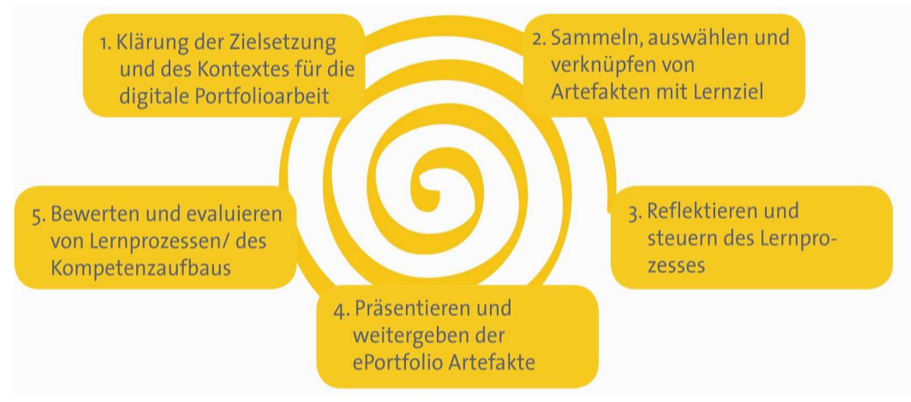
\includegraphics[width=0.7\linewidth]{e-portfolio-prozesse-schaffert}
		\caption{Prozesse der Portfolio-Arbeit (Schaffert et al. 2007, S. 79)\cite{schaffert_e-portfolio-einsatz_2007}}
		\label{fig:e-portfolio-prozesse-schaffert}
	\end{figure}
	\begin{figure}[h]
		\centering
		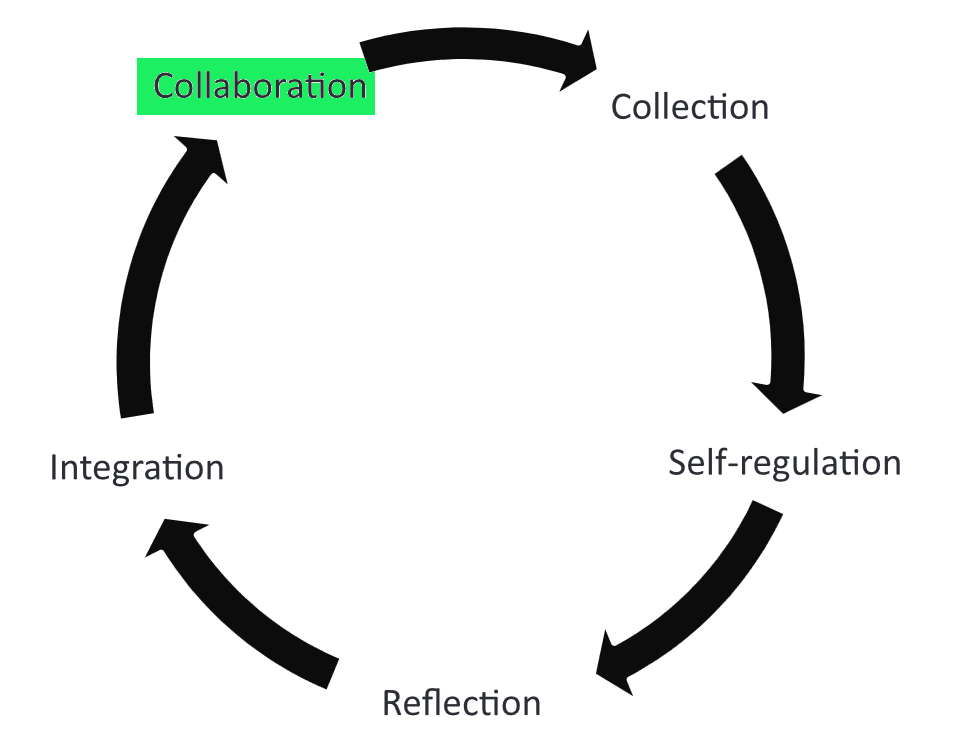
\includegraphics[width=0.5\linewidth]{cycle-of-documented-lifelong-learning-Jensen}
		\caption{cycle of documented lifelong learning (Jensen,Treuer 2014)\cite{jenson_defining_2014}}
		\label{fig:cycle-of-documented-lifelong-learning-jensen}
	\end{figure}
	\begin{figure}[h]
		\centering
		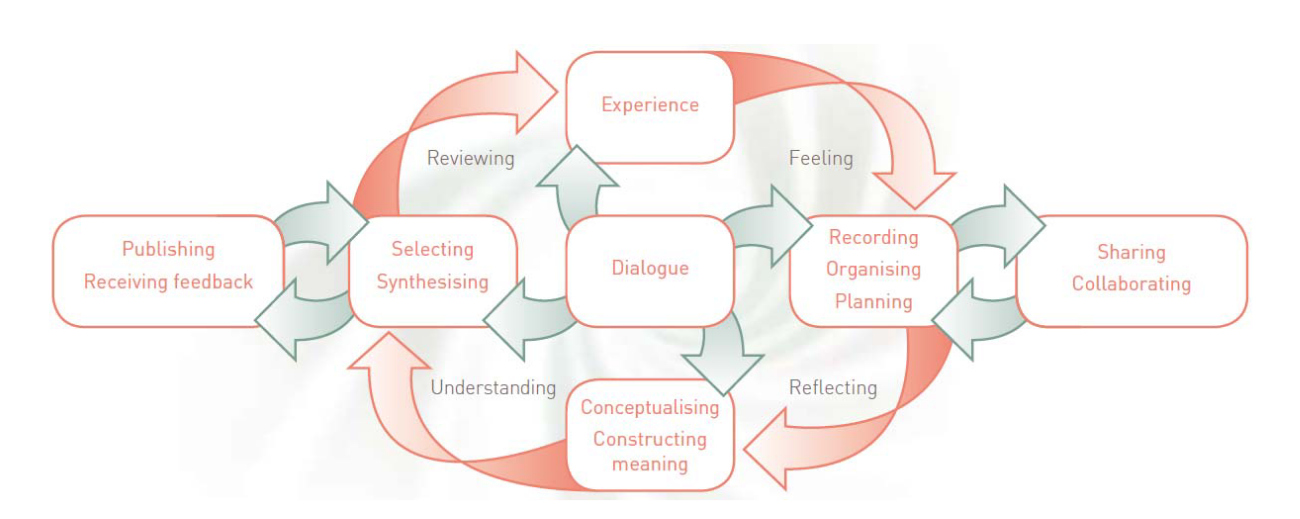
\includegraphics[width=0.8\linewidth]{model-of-e-portfolio-based-learning}
		\caption{A model of e-portfolio-based learning (JISC 2008, S. 9) \cite{jisc_effective_2008}}
		\label{fig:model-of-e-portfolio-based-learning}
	\end{figure}
	
	\pagebreak 
	
	\section*{Informationsmaterialien}
	
	Wiederhole dein Wissen über Latex oder nutze sonst im Notfall andere Editoren wie Word um PDF Dateien aus deinen Aufgaben und Artefakte, aber auch Scans, zu erstellen.
	
	\bibliographystyle{alpha}
	\bibliography{../eportfolio_lib}
	
	\pagebreak
	
	\section*{Einleitung}
	Sind meine Einschätzungen über mich selbst so gut? Was kann ich von anderen Lernen? Wie könnte ich meine Portfolioarbeit verbessern und effizienter gestalten? Wie fühle ich mich dabei anderen meine Artefakte zu präsentieren? Kann ich das auch nutzen um eine Bewerbung zu gestalten? Finde Dich hier zu erst in einer Gruppe von 4 bis 5 Personen zusammen.
	
	\section*{Aufgabenstellung}

	\begin{enumerate}
		\item In der Gruppe, solltet Ihr nun alle nacheinander vor an die Präsentierfläche und die Ergebnisse innerhalb 8 Minuten vorstellen. Danach sollen für 5 Minuten in einer Diskussionsrunde in der die anderen Mitglieder Feedback geben. Folgende Fragen sollen euch bei der Diskussion helfen. 
		\begin{enumerate}
			\item Was finde ich gut an dem Portfolio?
			\item Was würde ich an der Stelle des Vorstellenden besser machen?
		\end{enumerate}
		\item Nun bereite eine Ansicht vor, welche das öffentliche Internet/Andere Opal-Nutzer sehen sollen können. Halte Dich an den folgenden Leitfaden.
		\begin{enumerate}
			\item Eine öffentliche Sammelmappe für dein Studium bis jetzt und nutze ggf. diese Struktur:
			\begin{enumerate}
				\item 1 Zielsetzung
				\item 2 Artefakte
				\item 1 Reflexion
				\item 2 Artefakte
				\item 1 Evaluation(vorläufige)
			\end{enumerate}
		\end{enumerate}

	\end{enumerate}


\end{document}
